% !TEX TS-program = XeLaTeX
% use the following command:
% all document files must be coded in UTF-8
\documentclass[spanish]{textolivre}
% build HTML with: make4ht -e build.lua -c textolivre.cfg -x -u article "fn-in,svg,pic-align"

\journalname{Texto Livre}
\thevolume{15}
%\thenumber{1} % old template
\theyear{2022}
\receiveddate{\DTMdisplaydate{2021}{9}{24}{-1}} % YYYY MM DD
\accepteddate{\DTMdisplaydate{2021}{11}{7}{-1}}
\publisheddate{\DTMdisplaydate{2022}{2}{2}{-1}}
\corrauthor{Javier Mella Norambuena}
\articledoi{10.35699/1983-3652.2022.36310}
%\articleid{NNNN} % if the article ID is not the last 5 numbers of its DOI, provide it using \articleid{} commmand
% list of available sesscions in the journal: articles, dossier, reports, essays, reviews, interviews
\articlesessionname{articles}
\runningauthor{Mella-Norambuena et al.} 
%\editorname{Leonardo Araújo} % old template
\sectioneditorname{Hugo Heredia Ponce}
\layouteditorname{Anna Izabella Pereira}

\title{Modelos predictivos basados en uso de analíticas de aprendizaje en educación superior: una revisión sistemática}
\othertitle{Modelos preditivos baseados no uso de analítica da aprendizagem no ensino superior: uma revisão sistemática}
\othertitle{Predictive models based on the use of learning analytics in higher education: a systematic review}

% if there is a third language title, add here:
%\othertitle{Artikelvorlage zur Einreichung beim Texto Livre Journal}

\author[1]{Javier Mella Norambuena \orcid{0000-0002-4288-142X} \thanks{Email: \url{javier.mella1988@gmail.com}}}
\author[2]{María Graciela Badilla-Quintana \orcid{0000-0002-1317-9228}
\thanks{Email: \url{mgbadilla@ucsc.cl}}}
\author[3]{Yaranay López Angulo \orcid{0000-0002-3331-6875} \thanks{Email: \url{yara13190@gmail.com}}}
\affil[1]{Universidad Católica de la Santísima Concepción, Programa de Doctorado en Educación, Concepción, Chile / Universidad Técnica Federico Santa María, Departamento de Ciencias, Concepción, Chile.}
\affil[2]{Universidad Católica de la Santísima Concepción, Centro de Investigación en Educación y Desarrollo, Concepción, Chile.}
\affil[3]{Universidad Santo Tomás, Facultad de Ciencias Sociales y Comunicaciones, Escuela de Psicología, Concepción, Chile / Universidad de Concepción, Departamento de Psicología, Facultad de Ciencias Sociales, Concepción, Chile.}

\addbibresource{article.bib}
% use biber instead of bibtex
% $ biber article

% used to create dummy text for the template file
\definecolor{dark-gray}{gray}{0.35} % color used to display dummy texts
\usepackage{lipsum}
\SetLipsumParListSurrounders{\colorlet{oldcolor}{.}\color{dark-gray}}{\color{oldcolor}}

% used here only to provide the XeLaTeX and BibTeX logos
\usepackage{hologo}

% if you use multirows in a table, include the multirow package
\usepackage{multirow}

% provides sidewaysfigure environment
\usepackage{rotating}

% CUSTOM EPIGRAPH - BEGIN 
%%% https://tex.stackexchange.com/questions/193178/specific-epigraph-style
\usepackage{epigraph}
\renewcommand\textflush{flushright}
\makeatletter
\newlength\epitextskip
\pretocmd{\@epitext}{\em}{}{}
\apptocmd{\@epitext}{\em}{}{}
\patchcmd{\epigraph}{\@epitext{#1}\\}{\@epitext{#1}\\[\epitextskip]}{}{}
\makeatother
\setlength\epigraphrule{0pt}
\setlength\epitextskip{0.5ex}
\setlength\epigraphwidth{.7\textwidth}
% CUSTOM EPIGRAPH - END

% LANGUAGE - BEGIN
% ARABIC
% for languages that use special fonts, you must provide the typeface that will be used
% \setotherlanguage{arabic}
% \newfontfamily\arabicfont[Script=Arabic]{Amiri}
% \newfontfamily\arabicfontsf[Script=Arabic]{Amiri}
% \newfontfamily\arabicfonttt[Script=Arabic]{Amiri}
%
% in the article, to add arabic text use: \textlang{arabic}{ ... }
%
% RUSSIAN
% for russian text we also need to define fonts with support for Cyrillic script
% \usepackage{fontspec}
% \setotherlanguage{russian}
% \newfontfamily\cyrillicfont{Times New Roman}
% \newfontfamily\cyrillicfontsf{Times New Roman}[Script=Cyrillic]
% \newfontfamily\cyrillicfonttt{Times New Roman}[Script=Cyrillic]
%
% in the text use \begin{russian} ... \end{russian}
% LANGUAGE - END

% EMOJIS - BEGIN
% to use emoticons in your manuscript
% https://stackoverflow.com/questions/190145/how-to-insert-emoticons-in-latex/57076064
% using font Symbola, which has full support
% the font may be downloaded at:
% https://dn-works.com/ufas/
% add to preamble:
% \newfontfamily\Symbola{Symbola}
% in the text use:
% {\Symbola }
% EMOJIS - END

% LABEL REFERENCE TO DESCRIPTIVE LIST - BEGIN
% reference itens in a descriptive list using their labels instead of numbers
% insert the code below in the preambule:
%\makeatletter
%\let\orgdescriptionlabel\descriptionlabel
%\renewcommand*{\descriptionlabel}[1]{%
%  \let\orglabel\label
%  \let\label\@gobble
%  \phantomsection
%  \edef\@currentlabel{#1\unskip}%
%  \let\label\orglabel
%  \orgdescriptionlabel{#1}%
%}
%\makeatother
%
% in your document, use as illustraded here:
%\begin{description}
%  \item[first\label{itm1}] this is only an example;
%  % ...  add more items
%\end{description}
% LABEL REFERENCE TO DESCRIPTIVE LIST - END


% add line numbers for submission
%\usepackage{lineno}
%\linenumbers

\begin{document}
\maketitle

\begin{polyabstract}
\begin{abstract}
Los métodos tradicionales de predicción del riesgo académico en ocasiones presentan limitaciones para la identificación oportuna, por otro lado, las Analíticas de Aprendizaje presentan ciertas ventajas. El objetivo de este estudio fue analizar características de los modelos predictivos basados en analíticas de aprendizaje en Educación Superior. Se realizó una revisión sistemática de las bases Web of Science, Scopus y Eric usando las palabras clave "analítica de aprendizaje" y "predicción". Se seleccionaron 12 investigaciones que cumplieron con los criterios de inclusión. Los resultados indicaron que el 100\% de los estudios buscaron predecir el rendimiento académico, se incluyen variables de analíticas, sociodemográficas y sociocognitivas como predictoras. El sistema de gestión de aprendizaje más usado fue Moodle de cursos \emph{blended learning} y online. Los estudios se desarrollaron principalmente en Europa; las muestras fueron de hasta 500 participantes de Ingeniería y Tecnología. El tipo de análisis más frecuente fue regresión en software R y SPSS. La mayoría logró un modelo de predicción grande (R2 > .30). Se concluye que la construcción actual de modelos de predicción de abandono universitario posee importantes limitaciones.

\keywords{Modelo predictivo \sep Analítica de aprendizaje \sep Educación superior \sep Revisión sistemática}
\end{abstract}

\begin{portuguese}
\begin{abstract}
Os métodos tradicionais de previsão de risco acadêmico às vezes apresentam limitações para identificação oportuna. Por outro lado, a Analítica da Aprendizagem (\textit{Learning Analytics}) apresenta certas vantagens. O objetivo deste estudo é analisar características de modelos preditivos baseados na análise da aprendizagem no Ensino Superior. Uma revisão sistemática dos bancos de dados Web of Science, Scopus e Eric foi conduzida usando as palavras-chave "análise de aprendizagem" e "predição". Foram selecionados doze estudos de pesquisa que preenchiam os critérios de inclusão. Os resultados indicam que 100\% dos estudos buscaram prever o desempenho acadêmico, incluindo variáveis analíticas, sociodemográficas e sociocognitivas como preditores. O sistema de gerenciamento de aprendizagem mais comumente utilizado foi o Moodle para aprendizagem combinada e cursos \textit{on-line}. Os estudos foram realizados principalmente na Europa, sendo as amostras de até 500 participantes de Engenharia e Tecnologia. O tipo de análise mais frequente foi a regressão nos softwares R e SPSS. A maioria conseguiu um grande modelo de previsão (R2 > .30). Conclui-se que a atual construção de modelos de previsão de abandono escolar tem limitações importantes.

\keywords{Modelo preditivo \sep Analítica da aprendizagem \sep Educação superior \sep Revisão sistemática}
\end{abstract}
\end{portuguese}

\begin{english}
\begin{abstract}
Traditional prediction methods are  time-consuming and limited in identifying students at academic risk in a timely manner. On the other hand, Learning Analytics has certain advantages. The aim of this study was to analyze characteristics of predictive models based on learning analytics in higher education. A systematic review of Web of Science, Scopus and Eric databases was conducted using the keywords "learning analytics" and "prediction". Twelve research studies that met the inclusion criteria were selected. The results indicated that 100\% of the studies sought to predict academic performance, including analytical, sociodemographic and sociocognitive variables as predictors. The most used learning management system was Moodle for blended learning and online courses. The studies were mainly developed in Europe; the samples  consisted of up to 500 participants from Engineering and Technology. The most frequent type of analysis was regression in R and SPSS softwares. Most achieved a large prediction model (R2 > .30). It was concluded that the current construction of dropout prediction models has important limitations.

\keywords{Predictive model \sep Learning analytics \sep Higher education \sep Systematic review}
\end{abstract}
\end{english}
% if there is another abstract, insert it here using the same scheme
\end{polyabstract}

\section{Introducción}\label{sec-intro}
Actualmente para implementar procesos de enseñanza-aprendizaje efectivos, y a gran escala se necesitan las Tecnologías de la Información y la Comunicación (TIC), especialmente en la Educación Superior \cite{zhang2020}. Con la expansión de la revolución digital y un rápido cambio en las tecnologías, los datos educativos aumentan a un ritmo vertiginoso \cite{hooda2020, nguyen2021}. En esta línea, la incorporación de entornos virtuales de aprendizaje (EVA), o sistemas de gestión de aprendizaje (LMS por su nombre en inglés), se introdujeron de manera importante en las universidades desde comienzos del siglo XXI \cite{rojascastro2017}. Un LMS es un paquete de software basado en la web que está diseñado para planificar, implementar y evaluar el aprendizaje, facilitar la interacción de los estudiantes, dar retroalimentación sobre el rendimiento y gestionar las actividades de los estudiantes. Las universidades usan los LMS, siendo los más comunes Moodle, Edmodo, Canvas, Schoology, Blackboard Learn \cite{zhang2020}.

El uso de entornos virtuales de aprendizaje genera una huella digital asociada a registros de entrada y acciones, entre otras, que aporta una gran cantidad de información acerca de las actividades de los usuarios \cite{kerimbayev2020}. Estos datos usualmente se les conoce como big data educacionales o big data a secas, que son entendidos como un conjunto de datos cuyo tamaño excede la capacidad del software tradicional para su captura, gestión y análisis \cite{picciano2012, tulasi2013}. El surgimiento de la huella digital trae consigo una serie de nuevas áreas de estudio, tales como las analíticas o la minería de datos educacionales acerca del comportamiento de los estudiantes en estos ambientes o sobre las interacciones que allí ocurren \cite{klasnja-milicevic2017}. En un contexto de alto interés por parte de las universidades para mejorar resultados de aprendizaje y éxito académico, la aparición de la analítica contribuye a la satisfacción de estas necesidades.

En los últimos años, las Analíticas de Aprendizaje (en delante AA) han ido incrementando progresivamente y emergieron como un campo separado de investigación. Las AA son una nueva herramienta tecnológica considerada como una práctica de minería de conjunto de datos de las instituciones de Educación Superior para generar inteligencia procesable a través de técnicas de modelado estadístico y predictivo con el propósito de mejorar la toma de decisiones, el resultado y éxito de los estudiantes \cite{hooda2020}. Los estudios sobre AA se pueden agrupar en tres períodos: 1) los estudios realizados hasta el 2010, 2) los estudios realizados entre 2011-2014 y 3) los estudios realizados desde el 2015 \cite{sahin2019}. Actualmente, su crecimiento ha sido reconocido en el campo de la investigación y se ha documentado ampliamente, donde herramientas analíticas sofisticadas son usadas para mejorar el aprendizaje y la educación, especialmente en los sistemas de gestión del aprendizaje \cite{cechinel2020}.

Las AA se comprenden como el uso, la evaluación, la obtención y el análisis de información estática y dinámica sobre los estudiantes y los contextos de aprendizaje, para el modelado, la predicción y la optimización de procesos de aprendizaje, entornos de aprendizaje, así como para la toma de decisiones educativas \cite{hooda2020}. Es decir, se entiende como la medición, recopilación, análisis y reporte de datos sobre los estudiantes y sus contextos, con el propósito de comprender y optimizar el aprendizaje y los entornos en los que ocurre y por tanto su objetivo es procesar datos educativos para ofrecer información significativa relacionada con los perfiles de los estudiantes, materiales de aprendizaje, y el contexto de aprendizaje \cite{nguyen2021}.

Las AA contribuyen a ayudar a Instituciones de Educación Superior (IES) en muchos aspectos del aprendizaje y la enseñanza utilizando los datos generados sobre los estudiantes y su experiencia de aprendizaje. Así, es posible convertir los datos sin analizar en información procesable que mejoran las decisiones relacionadas con la educación, informando y empoderando a las autoridades institucionales, académicos, estudiantes e investigadores de los problemas que se identifican mediante técnicas de minería de datos y aprovechar el juicio humano \cite{guerra2020, hooda2020}. Tradicionalmente, estas decisiones eran tomadas por autoridades universitarias basadas en presunciones e hipótesis, procesos que además consumen mucho tiempo y limitan su calidad \cite{hooda2020}.

Respecto a los fenómenos educativos clave a los cuales aportan las AA, y áreas más frecuentemente enfocadas por parte de los investigadores sobre su uso en IES, son los métodos para mejorar el desempeño, el comportamiento, predecir el rendimiento y la retención de los estudiantes, especialmente considerando que muchos estudiantes no completan sus cursos \cite{guerra2020}. En este contexto, las AA pueden proveer de información relevante como la identificación de estudiantes en riesgo, la posibilidad de construir un apoyo adaptativo en su viaje de aprendizaje o proporcionarles apoyo adicional para hacer frente a los problemas académicos, requisitos y expectativas \cite{ifenthaler2020b}. Las AA ayudan a comprender el comportamiento de estudio, permiten brindar retroalimentación personalizada, facilitan la comprensión por parte de los docentes de los procesos de aprendizaje de sus estudiantes y orientan al diseño diferenciado y específico de intervenciones \cite{ifenthaler2020b, sahin2019}. En este sentido, \textcite{zhang2020}, concluyó que las AA se pueden utilizar para predecir el éxito de los estudiantes y estimular mejores resultados durante el estudio.

Los modelos explicativos del éxito académico en la Educación Superior incluyen factores sociodemográficos de los estudiantes, por ejemplo género, origen étnico, antecedentes familiares; su capacidad cognitiva o rendimiento académico previo, como el promedio de notas; atributos individuales, como los  rasgos personales e influencias contextuales motivacionales o psicosociales; así como factores relacionados con el curso, como el aprendizaje activo, la atención, o factores ambientales relacionados con la integración académica y social de apoyo. La posibilidad de recopilar y almacenar datos para los factores mencionados anteriormente y combinarlos constituye una enorme posibilidad que en la actualidad permiten las AA \cite{ifenthaler2020b}.

Los sistemas de gestión del aprendizaje (SGA) suelen centrarse en la organización de cursos de los profesores e incluyen la gestión de los estudiantes en un entorno de aprendizaje en línea moderno. Las instituciones educativas utilizan sistemas tecnológicos como Moodle, Edmodo, Canvas, Schoology, Blackboard Learn, entre otros \cite{zhang2020}. Al acceder con una cuenta personal, la actividad de cada estudiante queda en un archivo de registro. Las AA básicamente buscan responder a preguntas como: de qué, por qué, quién y cómo, para la optimización de estos entornos de aprendizaje utilizando los SGA como fuentes de datos que ofrecen mucha información y recursos a los estudiantes, tutores, autoridades, instituciones, investigadores y diseñadores.

Aunque se ha evidenciado la importancia de las AA para evaluar y predecir el desempeño de los estudiantes, mejorar las prácticas de aprendizaje y enseñanza, y tomar decisiones más rápidas basadas en datos \cite{hooda2020} es un área del conocimiento que aún tiene varias limitaciones. Por ejemplo, el desarrollo de investigación es alto en países anglosajones pero es incipiente en la región latinoamericana \cite{cechinel2020} y autores como \textcite{ifenthaler2020b} señalan que se requiere ampliar la evidencia sobre la efectividad de intervenciones basadas en las AA. Para esto es importante conocer los modelos predictivos disponibles en el área.

Respecto a la sistematización de la literatura para identificar la productividad de las AA en contexto de educación superior, se han realizado algunas aproximaciones teóricas, pero estas se han focalizado en cuestiones relacionadas con facilitar el éxito del estudio en la continuación y finalización, del aprendizaje de los estudiantes \cite{ifenthaler2020a}, en la eficacia de las AA en la intervenciones en términos de retención de estudiantes o éxito académico \cite{larrabee2019}, y otras relacionadas con identificar los beneficios de utilizar las AA en la Educación Superior \cite{banihashem2018}.  Sin embargo, no se ha encontrado evidencia de sistematizaciones que identifiquen los modelos desarrollados y probados empíricamente basados en AA para explicar fenómenos en la Educación Superior. Por lo anterior, en este artículo se propone sistematizar la evidencia disponible sobre las AA que aporte información para responder a la siguiente pregunta de investigación: ¿qué características tienen los modelos predictivos basados en AA usados en Educación Superior? Los objetivos específicos son: (1) Determinar las características que tienen los modelos predictivos basados en AA en Educación Superior respecto de variables predictoras consideradas, fenómeno que busca explicar, tipo de LMS como fuente extracción de datos, tipo de modelo, software para el análisis y resultado del modelo; (2) Describir las características que tienen los participantes en los modelos predictivos que usan AA en Educación Superior.

\section{Método}
Para la revisión y selección de artículos, se utilizó la metodología de revisión sistemática basada en las directrices internacionales de PRISMA \cite{moher2015}, en dos procesos consecutivos. El primero tuvo por objetivo identificar la muestra de estudios y el segundo elaborar una matriz que da cuenta del protocolo de extracción de la información de los estudios para su posterior análisis.

\subsection{Proceso 1. Selección de la muestra de estudios}
El proceso de selección de los artículos implicó 5 fases específicas: identificación, duplicado, elegibilidad, selección y sesgo, las que se pueden apreciar en la \Cref{fig1}. La fase de identificación consistió en la búsqueda de artículos en las bases de datos Web of Science (WOS), Scopus y Eric usando como palabras clave “analíticas de aprendizaje” y “predicción” o “predictivo” en inglés, las cuales fueron validadas por 6 jueces expertos. El período de búsqueda no se restringió debido a lo acotado de los resultados en indagaciones preliminares. Se aplicaron los filtros proporcionados por cada base de datos. La exploración en las bases de datos y búsqueda de los estudios se realizó el 22 de mayo de 2021. La fase de duplicado implicó la eliminación de estudios repetidos dejando solo uno. La fase de cribado consistió en una revisión por el investigador principal y dos jueces independientes, a los cuales se les presentó como protocolo para llevar a cabo la eliminación de estudios en esta fase la descripción del objetivo de la revisión sistemática y las palabras clave que debían identificar en el título y resumen. Se eliminaron artículos que no contenían las palabras clave o no respondían al objetivo de la presente investigación. La etapa de selección implicó la descarga de los archivos en formato pdf de los estudios y la lectura completa para la aplicación de los criterios de exclusión previamente establecidos. Se incluyeron investigaciones empíricas cuantitativas sobre AA con diseños predictivos en estudiantes universitarios cuyos datos para el análisis fueron extraídos de LMS institucionales. El proceso completo de esta parte del método se puede observar en la \Cref{fig1}.

\begin{figure}[htbp]
 \centering
 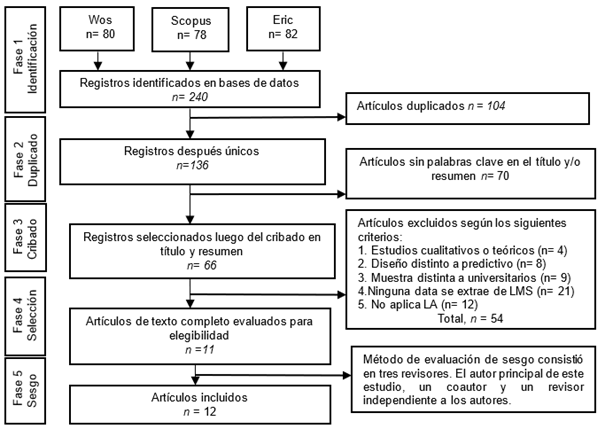
\includegraphics[width=0.8\textwidth]{36310-fig1.png}
 \caption{Flujograma de proceso completo identificación de estudios.}
 \label{fig1}
 \source{Elaboración propia.}
\end{figure}

\subsection{Proceso 2. Proceso de extracción de la información de la muestra de estudios seleccionados}
En la \Cref{tab1} se presenta la descripción de la información extraída de los estudios que fueron incluidos en esta revisión sistemática y en la \Cref{tab2} la matriz de datos.

\begin{table}[htpb]
\caption{Matriz explicativa de la información que fue extraída de la muestra de estudios seleccionados.}
\label{tab1}
\begin{tabular}{p{0.3\textwidth}p{0.6\textwidth}}
\toprule 
Información extraída & Descripción
\\ 
\midrule
ID & Identificador de la muestra de estudios seleccionados para la presentación de los resultados de esta RSL.
\\
Cita & Según formato de revista.
\\
Variable predicha (dependiente) & Variable que busca predecir el modelo hipotetizado.
\\
Variables predictoras (independiente) & Variables incluidas en los modelos predictivos correspondientes a las extraídas de los sistemas LMS institucionales.
\\
Tipo de LMS & Tipo de sistema de gestión del aprendizaje donde son extraídos los datos de analíticas de aprendizajes.
\\
Muestra & n: Corresponde al total de la muestra usada en el estudio. \newline país: corresponde al país de la institución donde se realizó el estudio.
\\
Modalidad de estudio & Formato de educación: Híbrida, \emph{blended-learning}, presencial.
\\
Tipo de modelo & Corresponde al análisis estadístico usado para probar el modelo hipotetizado (ejemplo, regresión, redes neuronales etc..).
\\
Software & Software estadístico con el que se realizó el tratamiento de los datos y análisis respectivos para probar el modelo hipotetizado.
\\
Resultado del modelo & Corresponde a los estadígrafos o coeficientes que dan cuenta del nivel de predicción del modelo (ejemplo: nivel de significancia dado por el valor p, porcentaje de predicción; coeficiente de determinación R2).
\\ 
\bottomrule
\end{tabular}
\source{Elaboración propia.}
\end{table}

\section{Resultados}
Se han separado los resultados según variable y se presentan a continuación.

\subsection*{Variable predicha en los modelos que usan AA}
En los modelos predictivos que usan AA, se identificó que en el 100\% de las investigaciones fue el rendimiento académico de los estudiantes la variable predicha.

\subsection*{Categorías de variables predictoras usadas en los modelos de AA}
Los resultados de esta revisión muestran que las variables incluidas en los modelos predictivos que usan AA en Educación Superior integran 3 grandes categorías: (1) variables sociodemográficas; (2) datos extraídos de LMS; y (3) variables sociocognitivas. El 100\% de los estudios incluyen diferentes datos de extracción de los LMS, mientras que dos investigaciones incluyeron además variables sociodemográficas (ID: 2, 10), y dos investigaciones incluyeron variables sociocognitivas (ID: 7, 11).

\subsection*{Resultados sobre el tipo de LMS}
El tipo de LMS identificado en el 92\% (n=11) de los estudios fue Moodle. Un estudio usó datos extraídos de la LMS Blackboard (ID: 11).

\subsection*{Resultados sobre la modalidad de estudio}
Las modalidades de estudio donde se desarrollaron las investigaciones corresponden a: 5 investigaciones en modalidad \emph{Blended Learning} (ID: 1, 2, 3, 4, 11); 5 corresponden a modalidad Online (ID: 12, 5, 8, 9, 10); y en dos estudios no se especificó la modalidad (ID: 7, 6).

\subsection*{Resultados sobre la muestra: país}
Los estudios se realizaron en nueve países distintos (Ver tabla 2) de los cuales fueron agrupados en categorías según continente (Ver \Cref{fig2}).

\begin{table}[htpb]
\caption{País de los participantes de los estudios.}
\label{tab2}
\centering
\begin{tabular}{lll}
\toprule 
País & ID & Frecuencia
\\ 
\midrule
Países bajos & 1,8,11 & 3
\\
Australia & 2,5 & 2
\\
Italia & 4 & 1
\\
España & 7 & 1
\\
Turquía & 12 & 1
\\
Taiwan & 3 & 1
\\
Israel & 9 & 1
\\
Ecuador & 6 & 1
\\
Estados Unidos & 10 & 1
\\ 
\bottomrule
\end{tabular}
\source{Elaboración propia.}
\end{table}

\begin{figure}[htbp]
 \centering
 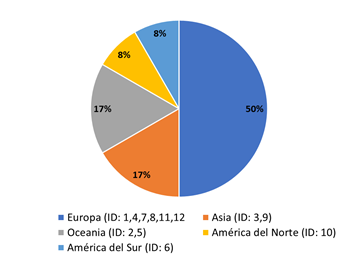
\includegraphics[width=0.5\textwidth]{36310-fig2.png}
 \caption{País de los participantes agrupados por continente.}
 \label{fig2}
 \source{Elaboración propia.}
\end{figure}

\subsection*{Resultados sobre la muestra total}
Para el tamaño muestral se establecieron 5 rangos (ver \Cref{fig3}), siendo el tamaño de muestra más usado en los estudios el rango entre 101 a 500 estudiantes (34\%).

\begin{figure}[htbp]
 \centering
 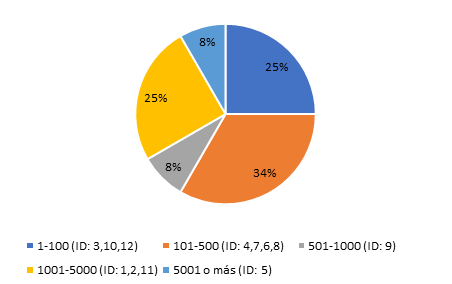
\includegraphics[width=0.6\textwidth]{36310-fig3.png}
 \caption{Rangos de tamaños de muestras usadas en los estudios.}
 \label{fig3}
 \source{Elaboración propia.}
\end{figure}

\subsection*{Resultados sobre la carrera}
En relación con las carreras que fueron parte de los estudios, dos investigaciones incluyeron carreras del área de la salud (ID: 7, 8). También se identificó un estudio que integró una carrera perteneciente al área de educación (ID: 4), un estudio que incluyó el área de economía (ID: 11), y otro estudio que incluyó una carrera del área de ingeniería. Además, en 7 investigaciones, no se especificaron qué carreras incluyeron (ID: 12, 1, 2, 3, 5, 9 y 10).

\subsection*{Resultados sobre la muestra: cursos}
Los cursos a los que pertenecían los estudiantes fueron clasificados según su correspondencia con las áreas OCDE (Ver \Cref{fig4}). La categoría más frecuente incluyó asignaturas del área de Ingeniería y Tecnología.

\begin{figure}[htbp]
 \centering
 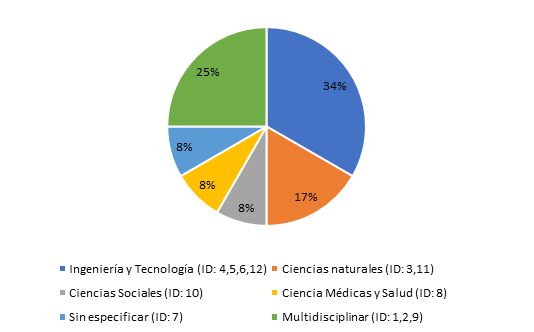
\includegraphics[width=0.8\textwidth]{36310-fig4.png}
 \caption{Curos por área OCDE.}
 \label{fig4}
 \source{Elaboración propia.}
\end{figure}

\subsection*{Resultados sobre el tipo de análisis}
Respecto a los tipos de análisis de predicción empleados en los estudios, el más frecuente fue el análisis de regresión lineal, se identificaron siete estudios (58\%) que los usaron en sus modelos predictivos (ID: 1, 2, 3, 7, 9, 10, 11), la red neuronal se usó en dos estudios (17\%) (ID: 5 y 6) y otros análisis identificados fueron la Distancias Levenshtein entre las cadenas relativas a trayectorias (ID: 4); y el Algoritmo KNN (ID: 8), ambos tipos de análisis usados en un estudio. Además, un estudio usó más de un tipo de análisis (ID: 12).

\subsection*{Resultados sobre el tipo de software}
Con relación al software usado para realizar los análisis de datos, los más frecuentemente usados fueron el software R (ID: 1, 6, 8) y el SPSS (ID: 2, 9 y 10), ambos usados por tres investigaciones respectivamente. Otros estudios usaron el software Python (ID: 5), Orange Data Mining software (ID: 12). Un estudio usó dos softwares (ID: 11), específicamente SPSS y Mplus. Tres investigaciones no especificaron el software que usaron para los análisis (ID: 3, 4).

\subsection*{Resultados de los modelos de predicción}
En los modelos identificados para predecir el rendimiento académico, se observó, en primer lugar, que en cuatro estudios hubo variabilidad en los rangos de varianza explicada según los modelos que fueron probados. En dos de los estudios esta variabilidad fue grande donde los modelos explicaron entre el 8\% y el 37\% (ID: 1) y el 7\% y 43\% de la varianza (ID: 11); mientras que otros dos la variabilidad de los modelos fue pequeña entre ellos, fluctuando entre 30\% y 38\% varianza explicada (ID: 3) y 88,3\% y un 90,9\% de la varianza explicada (ID: 8). En segundo lugar, se encontró un estudio que logró una predicción media dado que el modelo explicó un 21\% de la varianza. En tercer lugar, se observó que siete estudios lograron una predicción grande (ID: 4, 5, 6, 7, 9, 10, 12).

Los modelos que explican más de un 80\% de la varianza son investigaciones realizadas en cursos de modalidad online. Es posible observar que en cursos formativos en modalidad \emph{Blended Learning} los modelos predictivos explicaron entre el 7\% y el 77\% (ID: 1, 2, 3, 4, 11); mientras que en los cursos en modalidad Online explicaron entre un 32\% y un 90,9\% (ID: 5, 8, 8, 10 y 12). Este análisis muestra que los modelos predictivos basados en analítica de aprendizaje son más efectivos para explicar la variable de rendimiento académico en cursos universitarios de modalidad online.

\setlength\LTleft{-1.5in}
\setlength\LTright{-1in}
\begin{small}
\renewcommand{\arraystretch}{1.5}
\begin{longtable}{
    >{\raggedright\arraybackslash}p{0.008\textwidth}
    p{0.12\textwidth}
    p{0.1\textwidth}
    p{0.38\textwidth}
    p{0.15\textwidth}
    p{0.18\textwidth}
    p{0.16\textwidth}
    }
\caption{Matriz de extracción de información de la muestra de estudios seleccionados.}
\label{tab3}
\\
\toprule
ID & Cita & Variable predicha & Variables predictoras & Tipo LMS/ Modalidad & Muestra & Tipo de modelo / Software / Resultado del modelo
\\
\midrule
\arrayrulecolor[gray]{.7}
1 & \cite{conijn2017} & Rendimiento académico & Datos extraídos de LMS:
\begin{itemize}
\item[1] Número total de clics
\item[2] Número de sesiones en línea
\item[3] Tiempo total en línea
\item[4] Número de visitas a la página del curso
\item[5] Irregularidad del tiempo de estudio
\item[6] Irregularidad del intervalo de estudio
\item[7] Mayor periodo de inactividad (min)
\item[8] Tiempo hasta la primera actividad (min)
\item[9] Tiempo medio por sesión (min)
\item[10] Número de recursos consultados
\item[11] Número de enlaces vistos
\item[12] Número de páginas de contenido vistas
\item[13] Número de visitas a los debates
\item[14] Número total de mensajes de discusión
\item[15] Número de cuestionarios iniciados
\item[16] Número de intentos por cuestionario
\item[17] Número de cuestionarios aprobados
\item[18] Número de visitas a los cuestionarios
\item[19] Número de tareas enviadas
\item[20] Número de asignaciones (envío)
\item[21] Número de ediciones del wiki
\item[22] Número de visualizaciones del wiki
\end{itemize}	& Tipo de LMS: Moodle \newline Modalidad:
\emph{Blended Learning} & País: Países Bajos \newline N total: 4.989 \newline Carrera: No especifica \newline Curso: matemáticas, física y psicología & Tipo de modelo: Regresión lineal múltiple \newline Software: R \newline Resultado: Los modelos explicaron entre el 8\% y 37\% de la varianza.
\endfirsthead
\\
\midrule
2 & \cite{gasevic2016} & Éxito académico & Sociodemográficas
\begin{itemize}
\item[1] Edad
\item[2] Sexo (hombre/mujer);
\item[3] Estudiante internacional (sí/no);
\item[4] Idioma hablado en casa (inglés/idioma distinto del inglés);
\item[5] Lejanía del hogar (urbano/no urbano);
\item[6] Acceso a la universidad (estudiante a tiempo completo/parcial);
\item[7] Matriculación previa en el mismo curso (sí/no).
\item[8] acceso al inicio del curso (acceso temprano/no acceso al curso/acceso tardío)
\end{itemize}

Datos extraídos de LMS:
\begin{itemize}
    \item[1] Foros
    \item[2] Inicios de sesión en el curso recursos
    \item[3] Envío de archivos Turnitin, tareas, libro, cuestionarios, comentarios, mapa, aula virtual, lecciones y chat.	
\end{itemize} & Tipo de LMS: Moodle \newline Modalidad:
\emph{Blended Learning} & 	País: Australia \newline N total: 4134 \newline Carrera: No se especifica \newline Curso: contabilidad comunicación, informática, economía, diseño gráfico, marketing, matemáticas biología. & Tipo de modelo: Regresión lineal múltiple y modelos de regresión logística \newline Software: SPSS \newline
1.	Los modelos en promedio explicaron el 21\% de la varianza.
\\
\midrule
3 & \cite{lu2018} & Rendimiento académico final & Datos extraídos de LMS:
\begin{itemize}
\item[1] Número de días que muestra actividad
\item[2] Número de actividades que realiza
\item[3] Número de días que ve vídeos
\item[4] Número de vídeos que ve
\item[5] Número de vídeos que ve completamente
\item[6] Número de veces que hace clic en Buscar
\item[7] Número de vídeos en los que hace clic en "Pausa"
\item[8] Número de vídeos en los que hace clic en "Detener"
\item[9] Número de veces que hace clic en "Reproducir"
\item[10] Número de veces que un alumno hace clic en "Buscar hacia atrás"
\item[11] Número de veces que realiza prácticas en línea
\item[12] Número de unidades de Cálculo que un practica
\item[13] Número de días que practica en línea
\item[14] Suma de días de unidades de Cálculo practicadas
\item[15] Puntuación semanal de la práctica en línea
\item[16] Puntuación semanal de los deberes
\item[17] Puntuación semanal en los exámenes
\item[18] Número de veces que el alumno participa en la tutoría extraescolar
\item[*] por semana MOOCs en línea
\end{itemize} & Tipo de LMS: Open Edx) MOOCs, utiliza datos del lms y de aplicación OAS through Maple T.A \newline Modalidad:
\emph{Blended Learning} & País: Taiwán \newline N total: 59 \newline Carrera: No se especifica \newline Curso: Cálculo & Tipo de modelo: regresión de componentes principales \newline Software: No declara \newline Los modelos explicaron entre el 30\% y 38\% de la varianza.
\\
\midrule
4 & \cite{miranda2019} &  Resultados de aprendizaje & Datos extraídos de LMS: \newline 1. Ruta de navegación de los alumnos entre los contenidos. & Tipo de LMS: Moodle (moocs) \newline Modalidad: \emph{Blended Learning} & País: Italia \newline N total: 407 \newline Carrera: Ciencias de la Educación. \newline Curso: Ciencias básicas computacionales & Tipo de modelo: Distancias de Levenshtein entre las trayectorias \newline Software: No declara \newline 
Resultado:
1.	El porcentaje de estimación del modelo fue de 77\%.
\\
\midrule
5 & \cite{monllao_olive2020} & Rendimiento académico & Datos extraídos de LMS:
\begin{itemize}
\item[1] Valoraciones positivas en las entradas de la base de datos
\item[2] Valoraciones positivas en los mensajes del foro
\item[3] El estudiante intentó al menos un cuestionario
\item[4] Porcentaje de pruebas intentadas en el curso
\item[5] El alumno ha fallado un intento de cuestionario
\end{itemize} & Tipo de LMS: Moodle (moocs) \newline Modalidad:
Online & País: Australia \newline N total: 46.895 \newline Carrera: No aplica \newline Curso: Learn Moodle & Tipo de modelo: red neuronal \newline Software: Python \newline El porcentaje de precisión promedio del modelo fue de 88.81\%.  
\\
\midrule
6 & \cite{salgado2019} & Rendimiento académico & Datos extraídos de LMS:
\begin{itemize}
\item[1] Irregularidad del tiempo de estudio
\item[2] Irregularidad del intervalo de estudio
\item[3] Mayor periodo de inactividad
\item[4] Tiempo hasta la primera actividad (min)
\item[5] Tiempo promedio por sesión (min)
\item[6] Número de intentos por prueba
\item[7] Número de cuestionarios vistos
\item[8] Número de cuestionarios pasados
\item[9] Número de wiki vistas
\item[10] Número de consultas al profesor
\item[11] Participación en los foros
\item[12] Participación en chat
\item[13] Participación en video-colaboración
\item[14] Número de recursos vistos
\item[15] Número de enlaces vistos
\item[16] Número de páginas de contenido vistas
\item[17] Número de publicaciones de discusión vistas
\item[18] Número total de publicaciones de discusión
\item[19] Numero de cuestionarios iniciados
\item[20] Número de asignaciones enviadas
\item[21] Número de presentación vistas
\item[22] Número de ediciones en la wiki
\end{itemize} & Tipo de LMS: Moodle (moocs) \newline Modalidad:
No declara & País: Ecuador \newline N total: 300 \newline Carrera:  Sistemas \newline Cursos: Programación I, Programación II, Estructura de Datos, Programación Distribuida, Aplicaciones de Minería de Datos. & Tipo de modelo: red neuronal \newline Software: R \newline El porcentaje de precisión promedio del modelo fue de 75.28\%.
\\
\midrule
7 & \cite{saiz_manzanares2018} & Resultados finales de
aprendizaje & Datos extraídos de LMS:
\begin{itemize}
\item[1] Accesos a la información complementaria  
\item[2] Accesos a orientaciones para realizar actividad  
\item[3] Accesos a información sobre conceptos
\item[4] Accesos al feedback
\end{itemize}
Variables sociocognitivas: \newline Estrategias Metacognitivas
& Tipo de LMS: Moodle \newline Modalidad: No declara & País: España \newline N total: 122 \newline Carrera: Terapia Ocupacional y Enfermería \newline Curso: no especifica & Tipo de modelo: Regresión Lineal \newline Software: No declara \newline Los modelos en promedio explicaron en 64.1\% de la varianza.
\\
\midrule
8 & \cite{saqr2019} & Rendimiento académico	& Datos extraídos de LMS:
\begin{itemize}
\item[1] Temporalidad (participación diaria, participación semanal participaciones tempranas que corresponde al número de mensajes en el primer día de la semana; participaciones tardías; tendencias de participación a lo largo del día, la semana, el curso y todo el año).
\item[2] Duración de la conexión
\item[3] Número total de interacciones de un estudiante
\item[4] Tamaño de los mensajes.
\end{itemize} & Tipo de LMS: Moodle \newline Modalidad:
Online & País: Holanda \newline N total: 183 \newline Carrera: Odontología \newline Curso: Sistemas Corporales, Cirugía Dental, Neurociencia, y Principios de las Ciencias Odontológicas. & Tipo de modelo: KNN algorithm \newline Software: R \newline Los modelos explicaron entre el 88,3\% y un 90,9\% de la varianza.
\\
\midrule
9 & \cite{soffer2019} & Nota final del curso & Datos extraídos de LMS:
\begin{itemize}
\item[1] Actividad de vídeo en días
\item[2] Vídeos vistos (\%)
\item[3] Minutos de vídeo vistos (\%)
\item[4] Escribir en los foros
\item[5] Lectura de los mensajes del foro
\item[6] Entradas en la página de inicio del curso
\item[7] Entradas de la unidad de aprendizaje
\item[8] Entradas en la página media de la unidad
\item[9] Entradas de material adicional
\item[10] Tareas entregadas (\%)
\item[11] Entradas totales
\end{itemize} & Tipo de LMS: Moodle (moocs) \newline Modalidad:
Online & País: Israel \newline N total: 646 \newline Carrera: Programa de estudios complementarios \newline Cursos: curso en el ámbito de los estudios de Asia Oriental; curso en el ámbito de los estudios africanos; curso en Historia de la Mirada; curso en las Bases Celulares. & Tipo de modelo: análisis de regresión \newline Software: SPSS \newline El modelo final explicó el 33\% de la varianza.
\\
\midrule
10 & \cite{strang2016} & Rendimiento académico & Datos extraídos de LMS:
\begin{itemize}
\item[1] Entradas al curso,
\item[2] Lecciones vistas,
\item[3] Actividad de las tareas,
\item[4] Publicaciones en el foro
\end{itemize}

Variables demográficas para la
\begin{itemize}
\item[1] Edad
\item[2] Género
\item[3] Cultura de los estudiantes	
\end{itemize} & Tipo de LMS: Moodle (moocs) \newline Modalidad: Online & País: Estados Unidos \newline N total: 45 \newline Carrera: No especifica. \newline Curso: profesionalidad de división superior y gestión de recursos humanos	& Tipo de modelo: análisis de regresión pasos hacia atrás (stepwise backward) \newline Software: SPSS \newline El modelo final explicó el 32\% de la varianza.
\\
\midrule
11 & \cite{tempelaar2020} & Rendimiento académico & Datos extraídos de LMS:
\begin{itemize}
\item[1] BClicks como el número total de clics en BlackBoard.
\end{itemize}

Variables sociocognitivas:
\begin{itemize}
\item[1] Emociones de logro,
\item[2] Emociones epistémicas
\item[3] Objetivos de logro
\item[4] Motivación y compromiso
\item[5] Actitudes hacia el aprendizaje
\item[6] Enfoques del aprendizaje
\item[7] Motivaciones académicas
\end{itemize} & Tipo de LMS: blackboard \newline Modalidad: \emph{Blended Learning} & País: Países Bajos. \newline N total: 1080
estudiantes \newline Carrera: programa de negocios y economía \newline Curso: introducción a las matemáticas y la estadística & Tipo de modelo: regresión múltiple \newline Software: SPSS y Mplus \newline Los modelos explicaron entre el 7\% y 43\% varianza.
\\
\midrule
12 & \cite{akcapinar2019} & Rendimiento académico al final del trimestre & Datos extraídos de LMS:
\begin{itemize}
\item[1] El número total de sesiones
\item[2] La cantidad total de tiempo (en minutos) dedicado al aprendizaje
\item[3] El número de días diferentes en los que se registra el registro de aprendizaje
\item[4] El número total de visitas realizadas a los materiales de aprendizaje.
\item[5] El número total de visitas realizadas a las páginas de contenido.
\item[6] El número total de visitas realizadas a la página de notificación.
\item[7] El número total de visitas realizadas a la página de anuncios.
\item[8] El número total de visitas realizadas a la página de la publicación.
\item[9] El número total de visitas realizadas a la página de discusión.
\item[10] El número total de publicaciones creadas
\item[11] La cantidad promedio de tiempo (en segundos) dedicado a escribir publicaciones
\item[12] El número de días diferentes en los que se escriben las publicaciones.
\item[13] El número de etiquetas nuevas creadas al escribir una publicación.
\item[14] El número de etiquetas utilizadas en las publicaciones escritas.
\item[15] La cantidad de veces que se usa copiar y pegar al escribir publicaciones
\item[16] El número medio de pulsaciones de teclas que realiza el alumno mientras escribe una publicación
\item[17] El número medio de teclas de retroceso utilizadas por el alumno mientras escribiendo una publicación
\item[18]	La cantidad promedio de veces que la página perdió el foco al escribir una publicación.
\item[19] El número de puestos abiertos
\item[20] El número de comentarios creados
\item[21] El número de publicaciones calificadas
\item[22] El número de comentarios calificados
\item[23] El número total de respuestas escritas en el foro de discusión
\item[24] El número total de veces para abrir respuestas en el foro de discusión.
\item[25] El número de respuestas calificadas en el foro de discusión
\item[26] El número de preguntas calificadas en el foro de discusión	
\end{itemize} & Tipo de LMS: Moodle \newline Modalidad: Online & País: Turquía \newline N total: 76 \newline Carrera:  No se especifica \newline Curso: Hardware de Computadora & Tipo de modelo: Multimétodo (Naive Bayes, Árbol de clasificación, Bosque aleatorio, Red neuronal de máquinas de vectores de soporte, Reglas CN2) \newline Software: Orange data mining software (software de minería de datos de Orange)
\\
\arrayrulecolor{black}
\bottomrule
\source{Elaboración propia.}
\end{longtable}
\end{small}

\section{Discusión}
Este estudio se propuso realizar una revisión exhaustiva de la literatura sobre los modelos predictivos en la Educación Superior basado en el uso de AA. Se presenta la discusión de los resultados de cada información extraída de las investigaciones para responder al propósito de este estudio, además se presentan limitaciones y futuras líneas de investigación.

\subsection*{Discusión sobre las categorías de variables predictoras usadas en los modelos de AA}
Los resultados de esta revisión muestran que las variables incluidas en los modelos predictivos que usan AA en todos sus casos integran datos extraídos de las LMS institucionales, sin embargo, solo dos estudios incluyeron variables sociodemográficas y otros dos, variables sociocognitivas. Existe evidencia que los estudios en el campo de la AA que incluyen datos demográficos de los estudiantes y datos proporcionados por las LMS son identificadores eficaces del rendimiento "en riesgo". Sin embargo, la construcción de modelo con solo AA o aquellos que integran variables sociodemográficas no permiten una intervención personalizada para estos estudiantes \cite{zheng2020}. La información generada por estos modelos predictivos puede no ser adecuada para intervenciones pedagógicas debido a la incapacidad de explicar por qué los estudiantes muestran estos patrones de comportamiento. Para poder explicar el comportamiento de los estudiantes en las LMS se requiere incorporar variables sociocognitivas propias de la disposición al aprendizaje (por ejemplo, la autorregulación y las emociones) en los modelos convencionales de AA \cite{tempelaar2017}. Los modelos predictivos utilizados para los datos educativos siguen siendo inadecuados para ofrecer una imagen real del rendimiento académico de los estudiantes. Esto se debe a la falta de investigación sobre los modelos predictivos y los factores que afectan al rendimiento académico de los estudiantes \cite{zulkifli2019}. En definitiva, en el futuro, los modelos predictivos utilizados para el rendimiento académico de los estudiantes deberían tener en cuenta el último método de valoración de las evaluaciones basado en un sistema educativo moderno que haga hincapié en las habilidades blandas, las habilidades interpersonales y las capacidades de pensamiento de alto nivel.

\subsection*{Discusión sobre el tipo de LMS}
En relación con los tipos de LMS en la mayoría de los estudios se usó Moodle y solo uno usó Blackboard. Uno de los elementos importantes de un LMS es la capacidad de mejorar de forma óptima la calidad del aprendizaje y aplicar un sistema de aprendizaje interactivo. Una revisión sistemática se propuso analizar las características de flexibilidad, facilidad de uso y accesibilidad de diferentes LMS que pueden utilizarse para los procesos de enseñanza y aprendizaje en el contexto de las instituciones de educación superior \cite{kasim2016}. Los resultados identificaron 6 LMS diferentes, donde tres de ellos eran de código abierto (Moodle, Sakai y ATutor), mientas que otras tres eran comerciales (Blackboard, SuccessessFactors y Sum Total). Esto podría explicar por qué en los estudios identificados en la presente revisión, el LMS más frecuente fue Moodle y solo un estudio usó un LMS comercial, además, este último tiene menos disponibilidad de características para los usuarios. Específicamente el LMS Moodle se caracteriza por: (1) basado en la nube, (2) flexible, (3) fácil de usar, (4) capaz de integrarse con otros sistemas, (5) accesible. (6) uso amigable, (7) interacción sincrónica y asincrónica, (8) posibilidad de ver quién está en línea, (9) espacio personal para el borrador y diarios, así como para gestionar la información personal y privada, y (10) permite enviar y recibir mensajes personales con otros usuarios; sin embargo, el LMS Blackboard, solo dispone de las características 1, 2, 5, 6 y 7. Otra revisión teórica, con un propósito similar presentó una visión general  de las opciones de LMS disponibles para las universidades \cite{dobre2015}. Según los antecedentes descritos, aunque un número importante de universidades usa el LMS Blackboard, este ha comenzado a enfrentarse desde 2002 a una competencia muy fuerte, especialmente de otros LMS comerciales (Canvas, Desire2Learn), así como de LMS de código abierto (Moodle y Sakai). Los LMS comerciales pueden ser fáciles de desarrollar y utilizar, pero tienen un costo elevado; por otra parte, los LMS de código abierto son gratuitos, pero el costo de mantenimiento y mejora son elevados. En definitiva, el factor crucial que influye en la satisfacción de los estudiantes es que las características disponibles en un LMS satisfagan sus necesidades y faciliten su uso. En el caso de los investigadores es importante que los LMS permitan integrar acciones que faciliten el monitoreo del comportamiento de los estudiantes en las plataformas, lo que permitirá extraer información valiosa para predecir su rendimiento y consecuentemente disponer de esta información oportunamente para desplegar acciones de prevención de un rendimiento insuficiente. Finalmente, la efectividad y eficiencia de un LMS puede identificar y ayudar a resolver problemas potenciales \cite{kadir2016}.

\subsection*{Discusión sobre la modalidad de estudio}
Los resultados de esta revisión evidenciaron que las modalidades de estudio donde se desarrollaron las investigaciones corresponden a \emph{Blended Learning} y Online. Llama la atención que ninguno de los estudios se realizó en estudiantes de carreras en modalidad presencial, es decir, en carreras de clases convencionales. Estas, si bien se realizan en la interacción misma del aula presencial, en general, cuentan con una plataforma basada en LMS de los cursos que están desarrollando los estudiantes en un determinado semestre. La investigación previa describe la enseñanza tradicional en el aula como aquella basada en técnicas de enseñanza monótonas y que carece de interacción, por lo que los estudiantes pierden la curiosidad por comprender el propósito de estudiar \cite{priyaadharshini2020}. Los estudiantes esperan nuevas técnicas de enseñanza, asignaciones digitales y modelos de evaluación desafiantes. En la educación superior, se han introducido varios procesos nuevos de enseñanza-aprendizaje para motivar a los estudiantes y fomentar la práctica del autoaprendizaje, lo que facilita el desarrollo de mejores habilidades y conocimientos. Quizás es por esto, que este estudio no identificó investigaciones que usan AA en este ambiente presencial de aprendizaje. Sin embargo, con las diversas innovaciones en las TIC para la educación superior, el aprendizaje basado en diferentes métodos que incluyen el uso de las LMS se reconoce como una de las estrategias innovadoras de enseñanza-aprendizaje que han ido ganando interés en las universidades tradicionales. Por lo anterior, es esperable que las AA sean parte de las carreras que se desarrollan en la presencialidad, dado que como se ha avanzado, cuentan de igual forma con apoyo de diferentes LMS desde donde es posible extraer información de sus trayectorias académicas. Con el avance de la tecnología educativa y la necesidad de involucrar a los estudiantes del siglo XXI en las metas de aprendizaje, se requiere modificar el paradigma del aula de educación superior integrando los nuevos estilos de enseñanza innovadores que implican el uso de las TIC, contribuyendo a que los procesos de enseñanza-aprendizaje se agilizan con aulas inteligentes equipadas con actividades colaborativas donde los docentes aprovechan las herramientas TIC disponibles en los LMS y diferentes servicios en línea de los cursos disponibles de forma gratuita para las carreras en la educación superior \cite{srimadhaven2020}.

\subsection*{Discusión sobre la muestra: país}
La presente revisión mostró que los estudios de AA se han desarrollado principalmente en Europa mientas que en otras regiones del mundo cómo Oceanía, América y Asia es incipiente y en África no se identificaron estudios, esto coincide con una investigación previa que ha advertido como las estrategias actuales de diseño de aprendizaje se han situado dentro de instituciones específicas en Europa \cite{mittelmeier2018}. Aunque pudiera señalarse de forma clara que se recomienda el incremento de las AA en las diferentes regiones del mundo, se debe tener presente que los diferentes recursos tecnológicos adoptados por las universidades permiten a los docentes diseñar experiencias de aprendizaje con propósitos específicos para los estudiantes; estos tienen un sentido según los diversos contextos institucionales y culturales y de qué manera, lo que implica la necesidad de evaluar críticamente la relevancia y adecuación de la implementación de AA considerando las diferentes realidades \cite{zabolotniaia2020}. Por otra parte, autores han señalado el problema de las brechas en el desempeño de las instituciones de educación superior de África, identifica inmensas barreras estructurales y tecnológicas para la transformación efectiva y profunda de la enseñanza y el aprendizaje y que a su vez logren satisfacer las necesidades emergentes de equidad y acceso \cite{lusigi2019}. Con estos dos antecedentes discutidos, el desarrollo de estudios basados en AA en las diferentes regiones del mundo tiene un curso natural inherente a sus disposiciones y accesos tecnológicos.

\subsection*{Discusión sobre el tamaño de las muestras}
En cuanto a los tamaños muestrales usados en los estudios, se identificó que el rango de mayor frecuencia fue entre 101 a 500 estudiantes. Considerando que las AA son parte de las Ciencias de Datos y de lo conocido como big data, era esperable que las muestras más frecuentes fueran de tamaño grande, sin embargo, fue de un tamaño típico y propio de análisis de datos tradicionales \cite{wibawa2021}. Una posible explicación de esto es que los estudios implementaron un tipo de análisis predictivo, que tiene por propósito determinar qué variables explican en este caso el rendimiento académico de los estudiantes, y para ello requieren considerar varios aspectos específicos para que el modelo propuesto logre un nivel de predicción alto, y en este sentido, muestras grandes pueden implicar una variabilidad en las características de estas y por tanto un modelo resultante de baja predicción.

\subsection*{Discusión sobre la carrera y asignatura}
Este estudio reveló que más de la mitad de las investigaciones no especifica la carrera de los participantes. Los estudios que sí informaron la carrera señalan a las pertenecientes al área de educación, salud, economía e ingeniería. Por otra parte, se observó respecto de la asignatura, que prácticamente todos los estudios la describen, mostrando que pertenecen principalmente a cursos sobre Ingeniería y Tecnología. Esto es esperable, dado que como se ha advertido por diferentes investigaciones, las tasas de abandono y reprobación en cursos de esta área son alto \cite{lazaro_alvarez2020}. Dado que la presente revisión seleccionó investigaciones cuyo propósito es predecir el éxito de los estudios, es coherente que la mayor frecuencia de cursos sea parte de esta área disciplinar, puesto que históricamente sus estudiantes muestran dificultades para alcanzar las exigencias académicas.

\subsection*{Discusión sobre el tipo de análisis}
Respecto de los tipos de análisis de predicción empleados en los estudios, el usado con más frecuencia fue el análisis de regresión lineal. Otros identificados que se usaron en menor medida fueron la red neuronal, la Distancias Levenshtein entre las cadenas relativas a trayectorias y el Algoritmo KNN. Una revisión sistemática tuvo por objetivo identificar los métodos de predicción del rendimiento académico de los estudiantes en la educación superior \cite{zulkifli2019}. Los autores refieren que los modelos predictivos pueden clasificarse en tres (clasificación, clúster y regresión), aunque cada grupo tiene varios métodos que se desarrollaron de acuerdo con sus respectivos objetivos. La clasificación es un método utilizado para identificar las categorías de grupos de nuevas observaciones conocidas en conjuntos de grupos existentes, los métodos de clasificación utilizados más frecuentes son: Clasificación de Bayes (BC), K-Vecino más cercano (KNN), máquina de vectores de soporte (SVM) y árboles de clasificación (CT). Los clústeres o conglomerados (agrupación) son un método que implica el proceso de dividir datos o poblaciones en grupos que tienen caracteres casi idénticos o patrones, pero difieren entre grupos, entre los métodos utilizados para la agrupación se encuentran: Análisis de componentes Principales (PCA), Clustering de K-medias (K-M C), y agrupación jerárquica (HC). El análisis de regresión es un proceso estadístico para estimar la relación entre las variables dependientes y las independientes. A través del modelo de regresión que se ha construido, la variable dependiente se puede predecir fácilmente utilizando la variable independiente deseada. Los resultados encontrados por estos investigadores evidenciaron que el método más frecuente usado es el de clasificación, seguido por el de regresión. Este resultado sería contradictorio al del presente estudio, que mostró a la regresión como el más usado. Esto se podría explicar, dado que la revisión que hicieron los investigadores corresponde a modelos predictivos convencionales. Es decir, no incluyen AA, donde ellos mismos discuten que hay métodos recientes que han incorporado diferentes elementos en sus métodos, como la minería de datos, que combina métodos entre aprendizaje automático, estadísticas y sistemas de bases de datos para identificar patrones en grandes conjuntos de datos. En el método de minería de datos predictivo, los modelos que utilizan el método de clasificación se han categorizado como aprendizaje supervisado definido como aprender a enseñar o entrenar máquinas para reconocer datos a través de buen etiquetado. Mientras tanto, la predicción mediante el uso de clúster es más conocido como aprendizaje no supervisado, en minería de datos el que se lleva a cabo mediante máquinas para reconocer datos no etiquetados, pero permitiéndoles utilizar algoritmos contra los datos sin orientación. Respecto de los métodos de regresión, resultan desafiante puesto que los datos deben ser cuantitativos, normalizados, sin datos extremos y sin multicolinealidad. Datos con valores y atributos extremos utilizados en relación con los demás conduce a un uso inadecuado de estimaciones. Además, la cantidad de muestreo de datos utilizado en el método de minería de datos debe ser grande para que se pueda generalizar a la población.

\subsection*{Discusión sobre el tipo de software}
Respecto del software usado para realizar los análisis de datos, los más frecuentemente usados fueron el software R y el SPSS. Existen muchas herramientas estadísticas que se utilizan en el análisis de datos. Cada herramienta tiene ventajas y desventajas y se ha hecho popular según la característica en la que ha destacado como costo, visualización, paquetes, estadísticas, capacidad de manejo de datos, gráficos y también el big data entre otros factores. Casi todas las áreas, incluyendo educación, han puesto énfasis en torno a la capacidad de hacer predicciones y descubrir patrones en datos. La ciencia de datos es el centro de esta revolución. Eso incluye minería de datos, aprendizaje automático y estadísticas metodologías para extraer conocimiento y apalancamiento de predicciones a partir de datos. El valor de las estadísticas radica en organizar, transformar y simplificación de datos. Para lograr esto, se requieren herramientas de análisis de datos estadísticos \cite{bansal2018}. En los entornos de LMS, el estudio de los datos a través de la analítica de big data es muy poderoso, especialmente para la toma de decisiones y el uso de datos estadísticos en este entorno rico en datos. Tanto Python como R pueden utilizarse para tomar decisiones que implican grandes datos. Por un lado, Python es perfecto para la enseñanza de la estadística en un entorno rico en datos. Por otro lado, aunque R es un poco más complicado, hay muchos programas personalizables \cite{colliau2021}. En definitiva, los resultados del presente estudio, si bien identifican al Software R en las investigaciones analizadas como uno de los softwares más empleados, en la misma frecuencia de uso se identificó el software SPSS, y de acuerdo a lo señalado en la literatura, es el software como menos propiedad para ser usado en big data \cite{bansal2018}.

\subsection*{Discusión sobre los modelos de predicción}
Respecto de la predicción de los modelos identificados para predecir el rendimiento académico, se observaron diferentes resultados en las investigaciones. Algunos no lograron un nivel mínimo de predicción para fenómenos de las ciencias sociales (R2 < .01), mientras que otros lograron una predicación grande (R2 < .30). Esta variedad en los resultados puede tener diferentes explicaciones. En primer lugar, podría deberse a que la AA para predecir fenómenos en educación, es una línea de investigación reciente y por tanto considera una disciplina emergente (Siemens, 2013). Lo anterior ha implicado la reciente exploración de modelos predictivos de fenómenos como el rendimiento académico o la deserción de los estudios. Los investigadores, por una parte, usan solo variables de AA en los modelos, mientras que otros, han incluido variables sociodemográficas, y otros variables sociocognitivas. Esto implica una integración de diferentes categorías de variables en los modelos que pudieran estar influyendo en el poder predictivo de estos. En segundo lugar, se dispone de diferentes modelos para realizar los análisis estadísticos, los cuales varían en sus procesos y consecuentemente en sus resultados de predicción. En tercer lugar, las muestras de los estudios fueron diversas en cuanto al tamaño y las carreras participantes.

Los métodos tradicionales de predicción consumen mucho tiempo y son incapaces de identificar un número similar de estudiantes en riesgo académico a tiempo. Los investigadores empiezan a explorar el uso de la AA para construir modelos de predicción del abandono que permitan identificar tempranamente aquellos estudiantes de riesgo y, a continuación, realizar intervenciones antes de que el estudiante en riesgo abandone \cite{zheng2020}. La AA busca mejorar los procesos de aprendizaje a través de mediciones sistemáticas del aprendizaje datos relacionados y para proporcionar retroalimentación informativa a estudiantes y profesores. Sin embargo, la construcción actual de modelos de predicción de abandono tiene aún importantes limitaciones \cite{zheng2020}.

Este estudio también reveló que los modelos predictivos basados en AA que son más efectivos para explicar la variable rendimiento académico en cursos universitarios son aquellos de modalidad online. Esto podría explicarse, dado que el comportamiento de estudio de quienes cursan este tipo de programas está principalmente concentrado en los LMS \cite{mubarak2021}. En cambio, en Modalidad \emph{Blended Learning}, el comportamiento de estudio depende solo en una parte de los LMS, pero otra se da en modalidad presencial, donde no es posible por medio de las AA hacer seguimiento de las diferentes interacciones y dinámicas de estudio.

Por lo anterior, es importante que en cursos \emph{blended learning} o presencial, donde los LMS son solo una parte o un apoyo de la formación del estudiantado, se incluyan otras formas de medición de sus procesos autorregulatorios del estudio (patrones de aprendizaje), que permitan mejorar la predicción del rendimiento. Como, por ejemplo, las clásicas escalas de autorreporte, donde es el mismo estudiante quien autoinforma las características de sus procesos de disposición al estudio, monitoreo y autoevaluación del mismo.

Resulta clave comprender la actividad de estudio y aprendizaje del estudiantado para implementar acciones que permitan oportunamente retroalimentar su desempeño y promover estrategias efectivas para mejorar en una siguiente actuación, tal y como lo ha evidenciado la investigación de la autorregulación del aprendizaje y engagement académico. Para esto, tal como recomienda la investigación, se requiere nuevas propuestas de gestión de datos en las instituciones de educación superior, que permitan superar estos desafíos generando un proceso estandarizado de recolección de datos por medio de LMS y de escalas de medición de otras variables como las sociocognitivas, que no son informada por las AA y su trayectoria en investigación han demostrado su efectividad para predecir el desempeño académico, que sumado a as AA permitirían obtener modelos predictivos consistentes.

La presente revisión sistemática de la literatura tiene algunas limitaciones a considerar. Se revisaron tres bases de datos, pero no se incluyó la base de datos Scielo; y además carece de un análisis estadístico de la explicación de los modelos. Por tanto, un futuro estudio podría por una parte ampliar la revisión de estudios sobre AA incluyendo otras bases de datos y además realizar un meta análisis para evidenciar por medio de un mecanismo de análisis estadístico la predicción efectiva de los modelos propuestos en los estudios.

\section{Conclusiones}
A partir de los resultados se pueden establecer las siguientes conclusiones: 1) las variables que se incluyen en los modelos predictivos del rendimiento académico en la Educación Superior requieren incluir no solo AA, sino también otras variables psicoeducativas para comprender mejor el fenómeno; 2) los datos de analíticas son extraídos de los LMS institucionales y en todos los estudios analizados se trató de programas \emph{blended learning} y online, por tanto, se requieren investigaciones de modelos predictivos que usen las AA en programas tradicionales de enseñanza universitaria; 3) las investigaciones sobre modelos predictivos en Latinoamérica son incipientes, se requieren investigaciones considerando las particularidades regionales; (4) finamente, el poder predictivo del rendimiento académico en modelos que incorporan las AA es grande y por tanto prometedores para avanzar en las problemáticas actuales de la Educación Superior como el rendimiento académico y la permanencia.

\section*{Agencia de Financiamiento}
Beca Doctorado Nacional Folio 21212274 de la Agencia Nacional de Investigación y Desarrollo de Chile (ANID).


\printbibliography\label{sec-bib}
% if the text is not in Portuguese, it might be necessary to use the code below instead to print the correct ABNT abbreviations [s.n.], [s.l.]
%\begin{portuguese}
%\printbibliography[title={Bibliography}]
%\end{portuguese}


%full list: conceptualization,datacuration,formalanalysis,funding,investigation,methodology,projadm,resources,software,supervision,validation,visualization,writing,review
\begin{contributors}[sec-contributors]
\authorcontribution{Javier Mella Norambuena}[conceptualization,datacuration,methodology,writing]
\authorcontribution{María Graciela Badilla}[conceptualization,investigation,supervision]
\authorcontribution{Yaranay López Angulo}[conceptualization,visualization,review]
\end{contributors}

\end{document}
